\section{Problem and Dataset}
\label{sec:assumption}
%\KZ{Don't use script size for your tables. You have plenty of space.}OK
% \JY{here we can add a picture related so that some space can be occupied.}
In this paper, we ask two research questions: 
\begin{enumerate}
\item Do pet dogs from different human language environments sound differently? 
\item If so, is their vocalization related to their host's language in any way? 
\end{enumerate}

To answer these questions, we construct a dataset ``EJShibaVoice'', 
which is composed of Shiba Inu vocal samples from Japanese and English language environments 
and their corresponding hosts speech. Additionally, each audio sample is also tagged with
metadata such as the begin and end timestamps, and the context under which the vocal sound is made.    
%Here scenes represent for the brief definition of what 
%a dog is doing. And each scene falls into one of the eight scenes set by us. 
Additionally, host's speech from the same video is extracted using a similar approach as we process dog vocalizations. This procedure will be described in detail in~\secref{sec:speechextraction}.

To ensure the high quality of the dataset, we develop a rigorous processing pipeline to extract pure dog sounds in a variety of environments, with little or no extraneous noises such as human speech or background music. We segment dog audio clips into minimal units, which is a full singular bark, for the purpose of fine-grained acoustic comparison between different language environments. 
We further provide detailed extraneous context for each vocal clip, as there are other variables other than language environments that could potentially influence dog's  sound, for example whether a dog is eating or playing, outdoor or indoor\cite{larranaga2015comparing, molnar2008classification}. We make this fine distinction on the context of the dog sounds so as to constrain confounding factors other than the linguistic environment of the dogs. Hereby, with the sound segmentation and context tagging, each clean singular vocalization has a corresponding context.


Next, we present the full data processing pipeline~(\figref{fig:methodpic}) 
for constructing the EJShibaVoice dataset. 

\begin{figure}[ht]
	\centering
\begin{subfigure}[t]{0.48\columnwidth}
        \centering
        
\includegraphics[width=0.98\columnwidth]{images/image0.jpg}
        \caption{source videos and tag language.}
        \label{fig:source}
\end{subfigure}
\begin{subfigure}[t]{0.48\columnwidth}
        \centering
        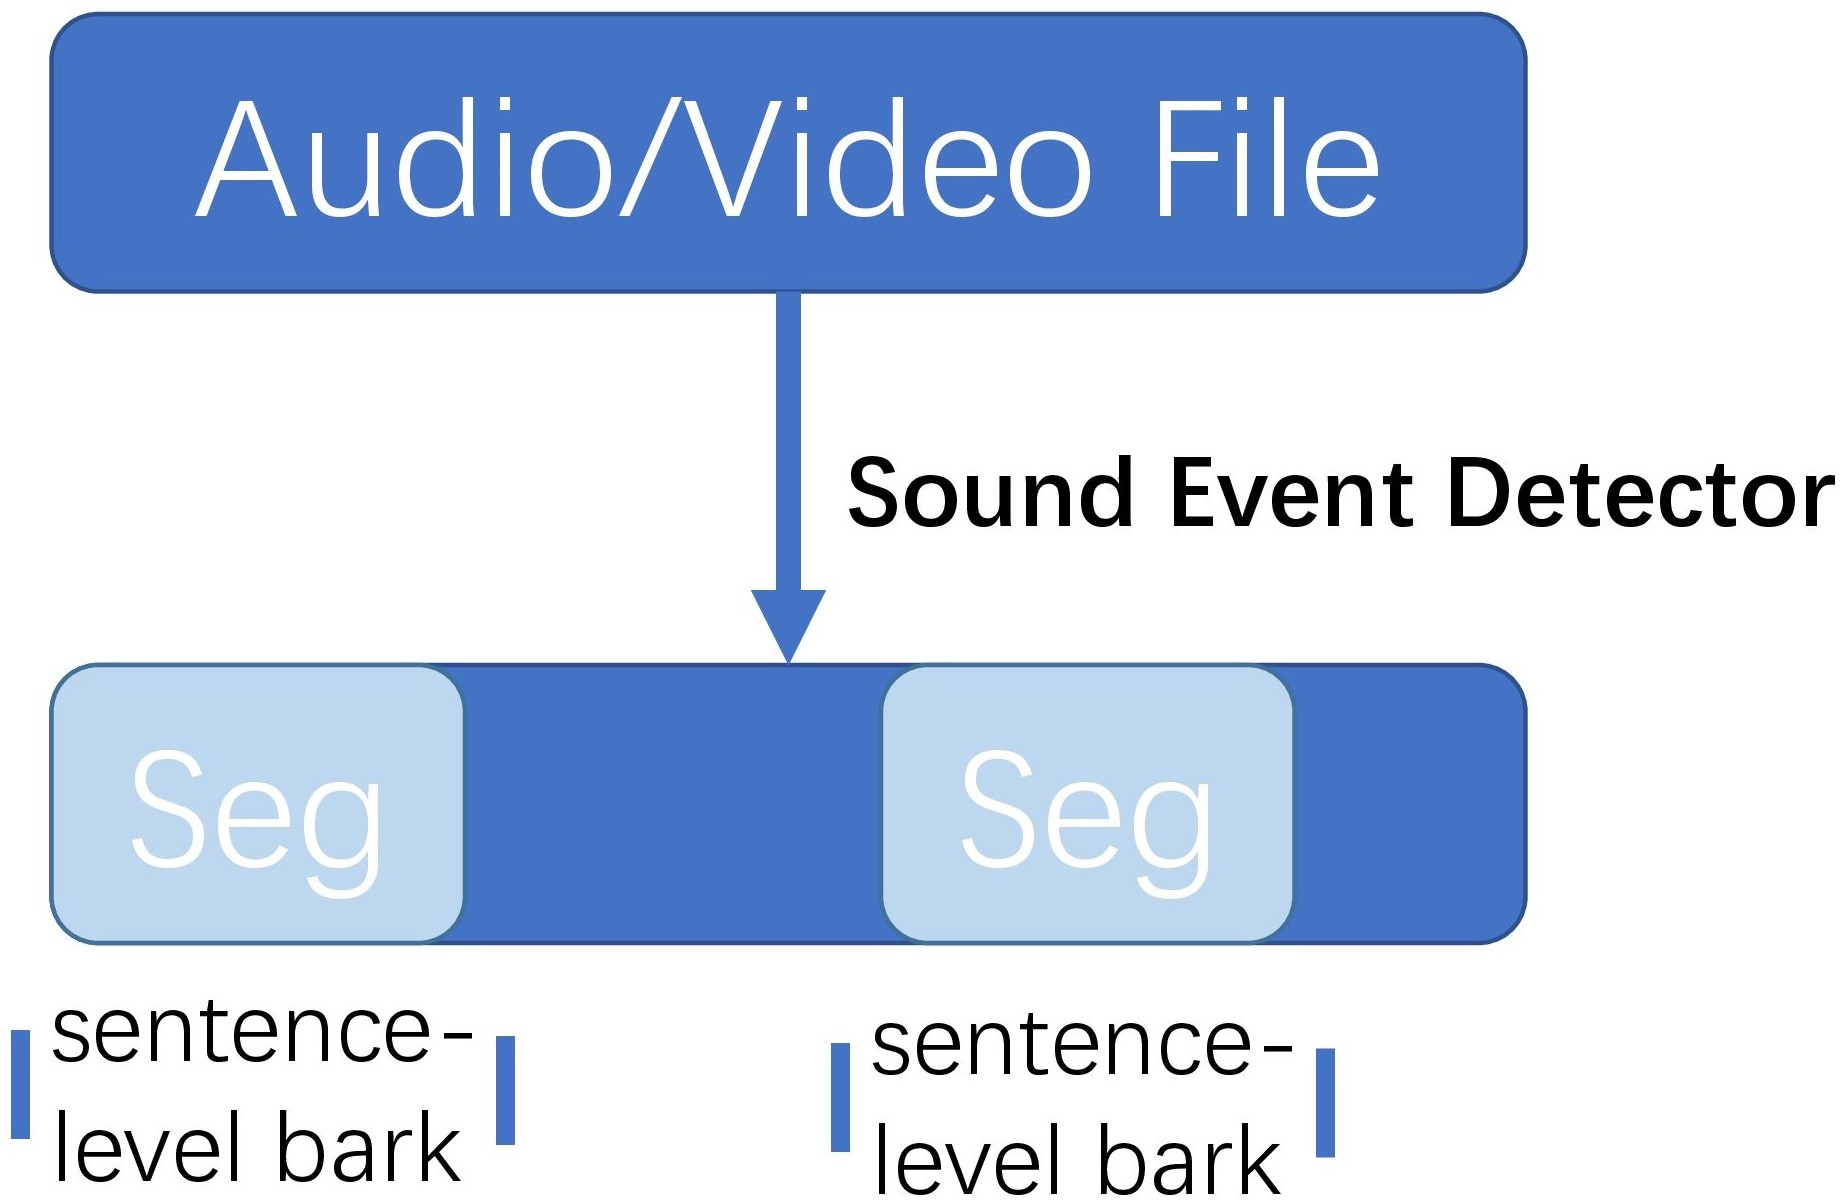
\includegraphics[width=0.7\columnwidth]{images/image1.jpg}
	\caption{sentence-level segmentations.}
        \label{fig:sentence}
\end{subfigure}
\begin{subfigure}[t]{0.48\columnwidth}
        \centering
        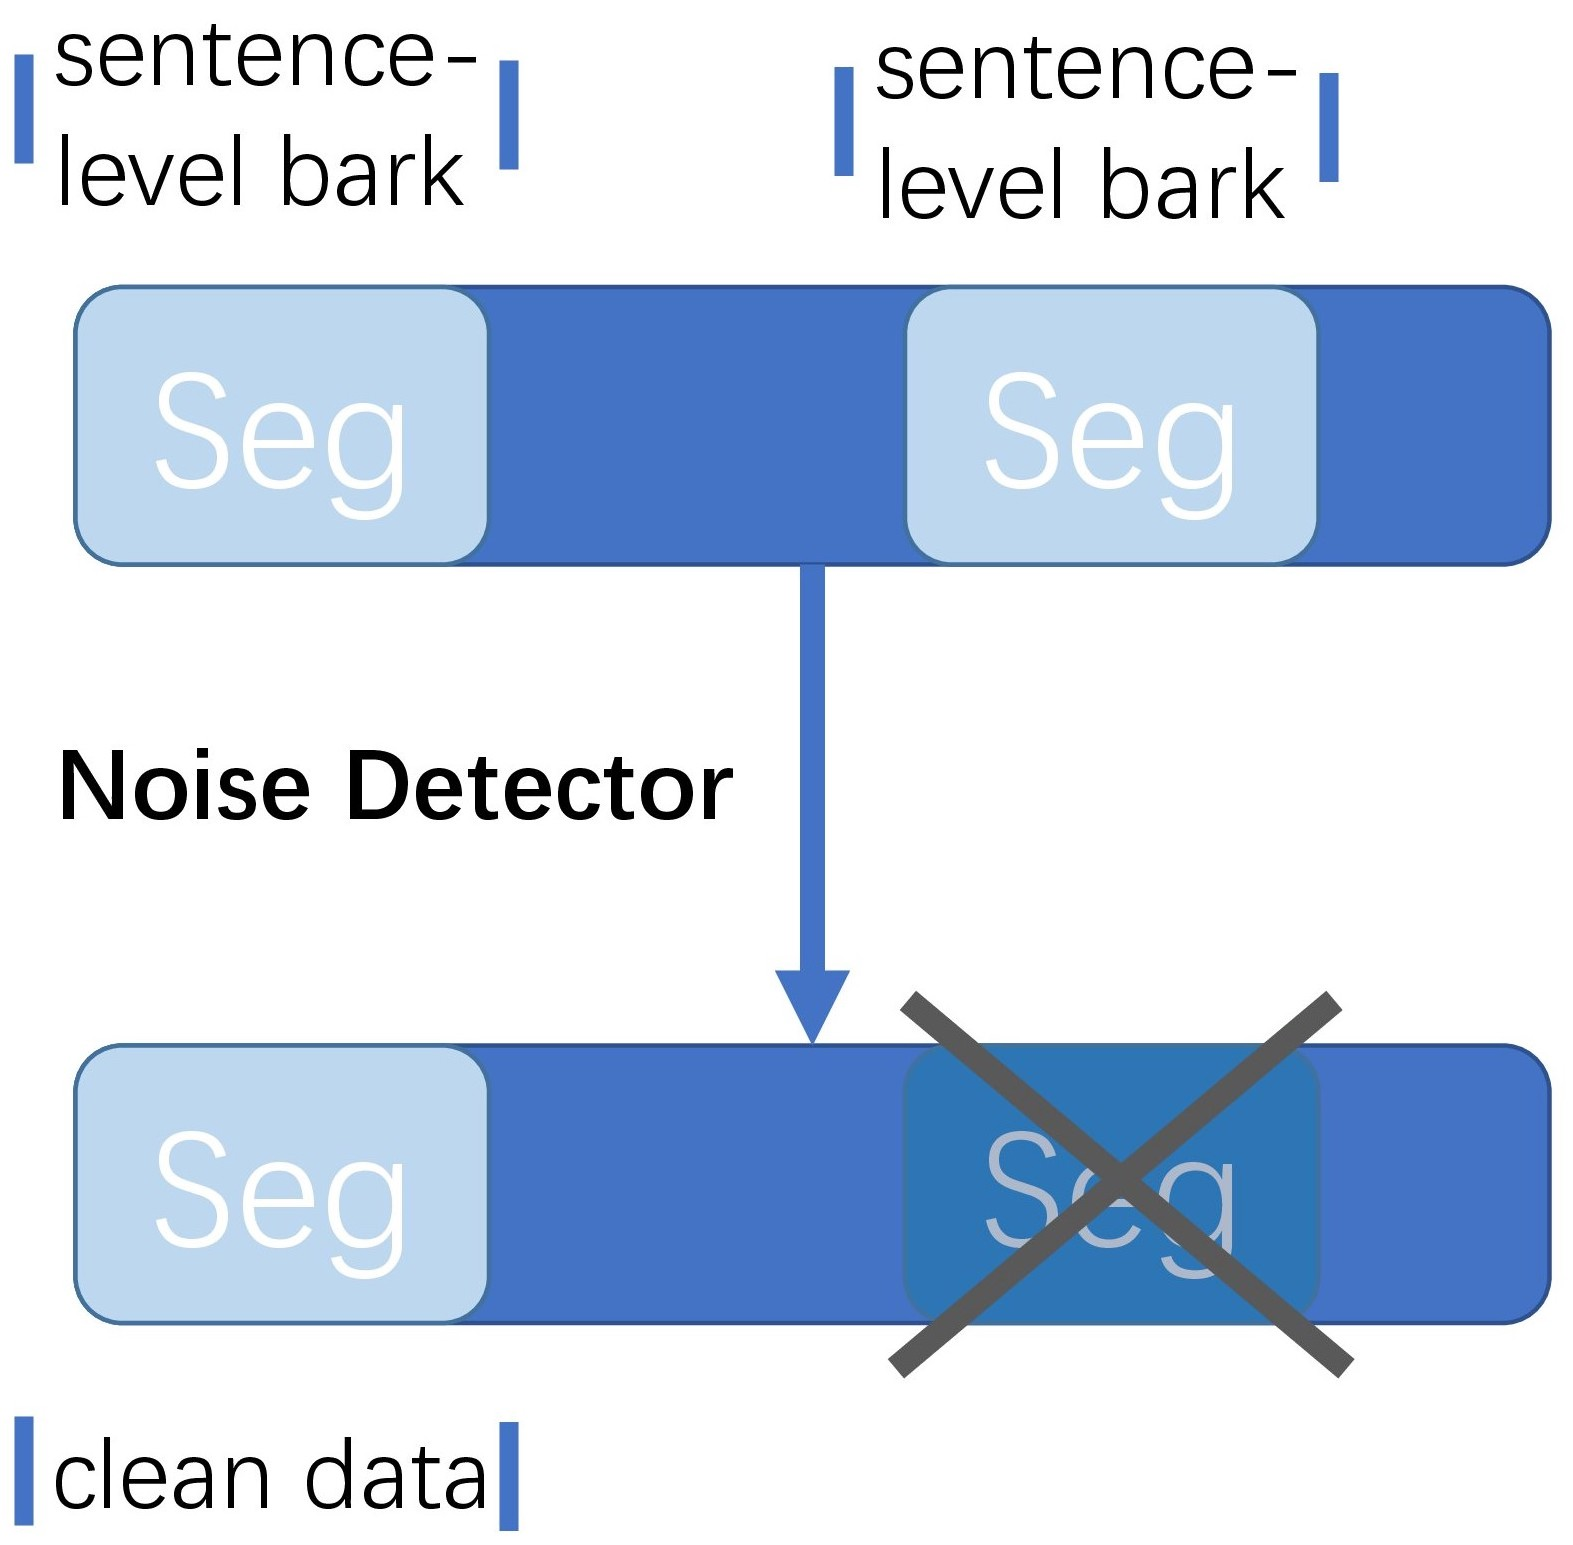
\includegraphics[width=0.7\columnwidth]{images/image2.jpg}
	\caption{clean data after noise removing.}
        \label{fig:clean}
\end{subfigure}
\begin{subfigure}[t]{0.48\columnwidth}
        \centering
        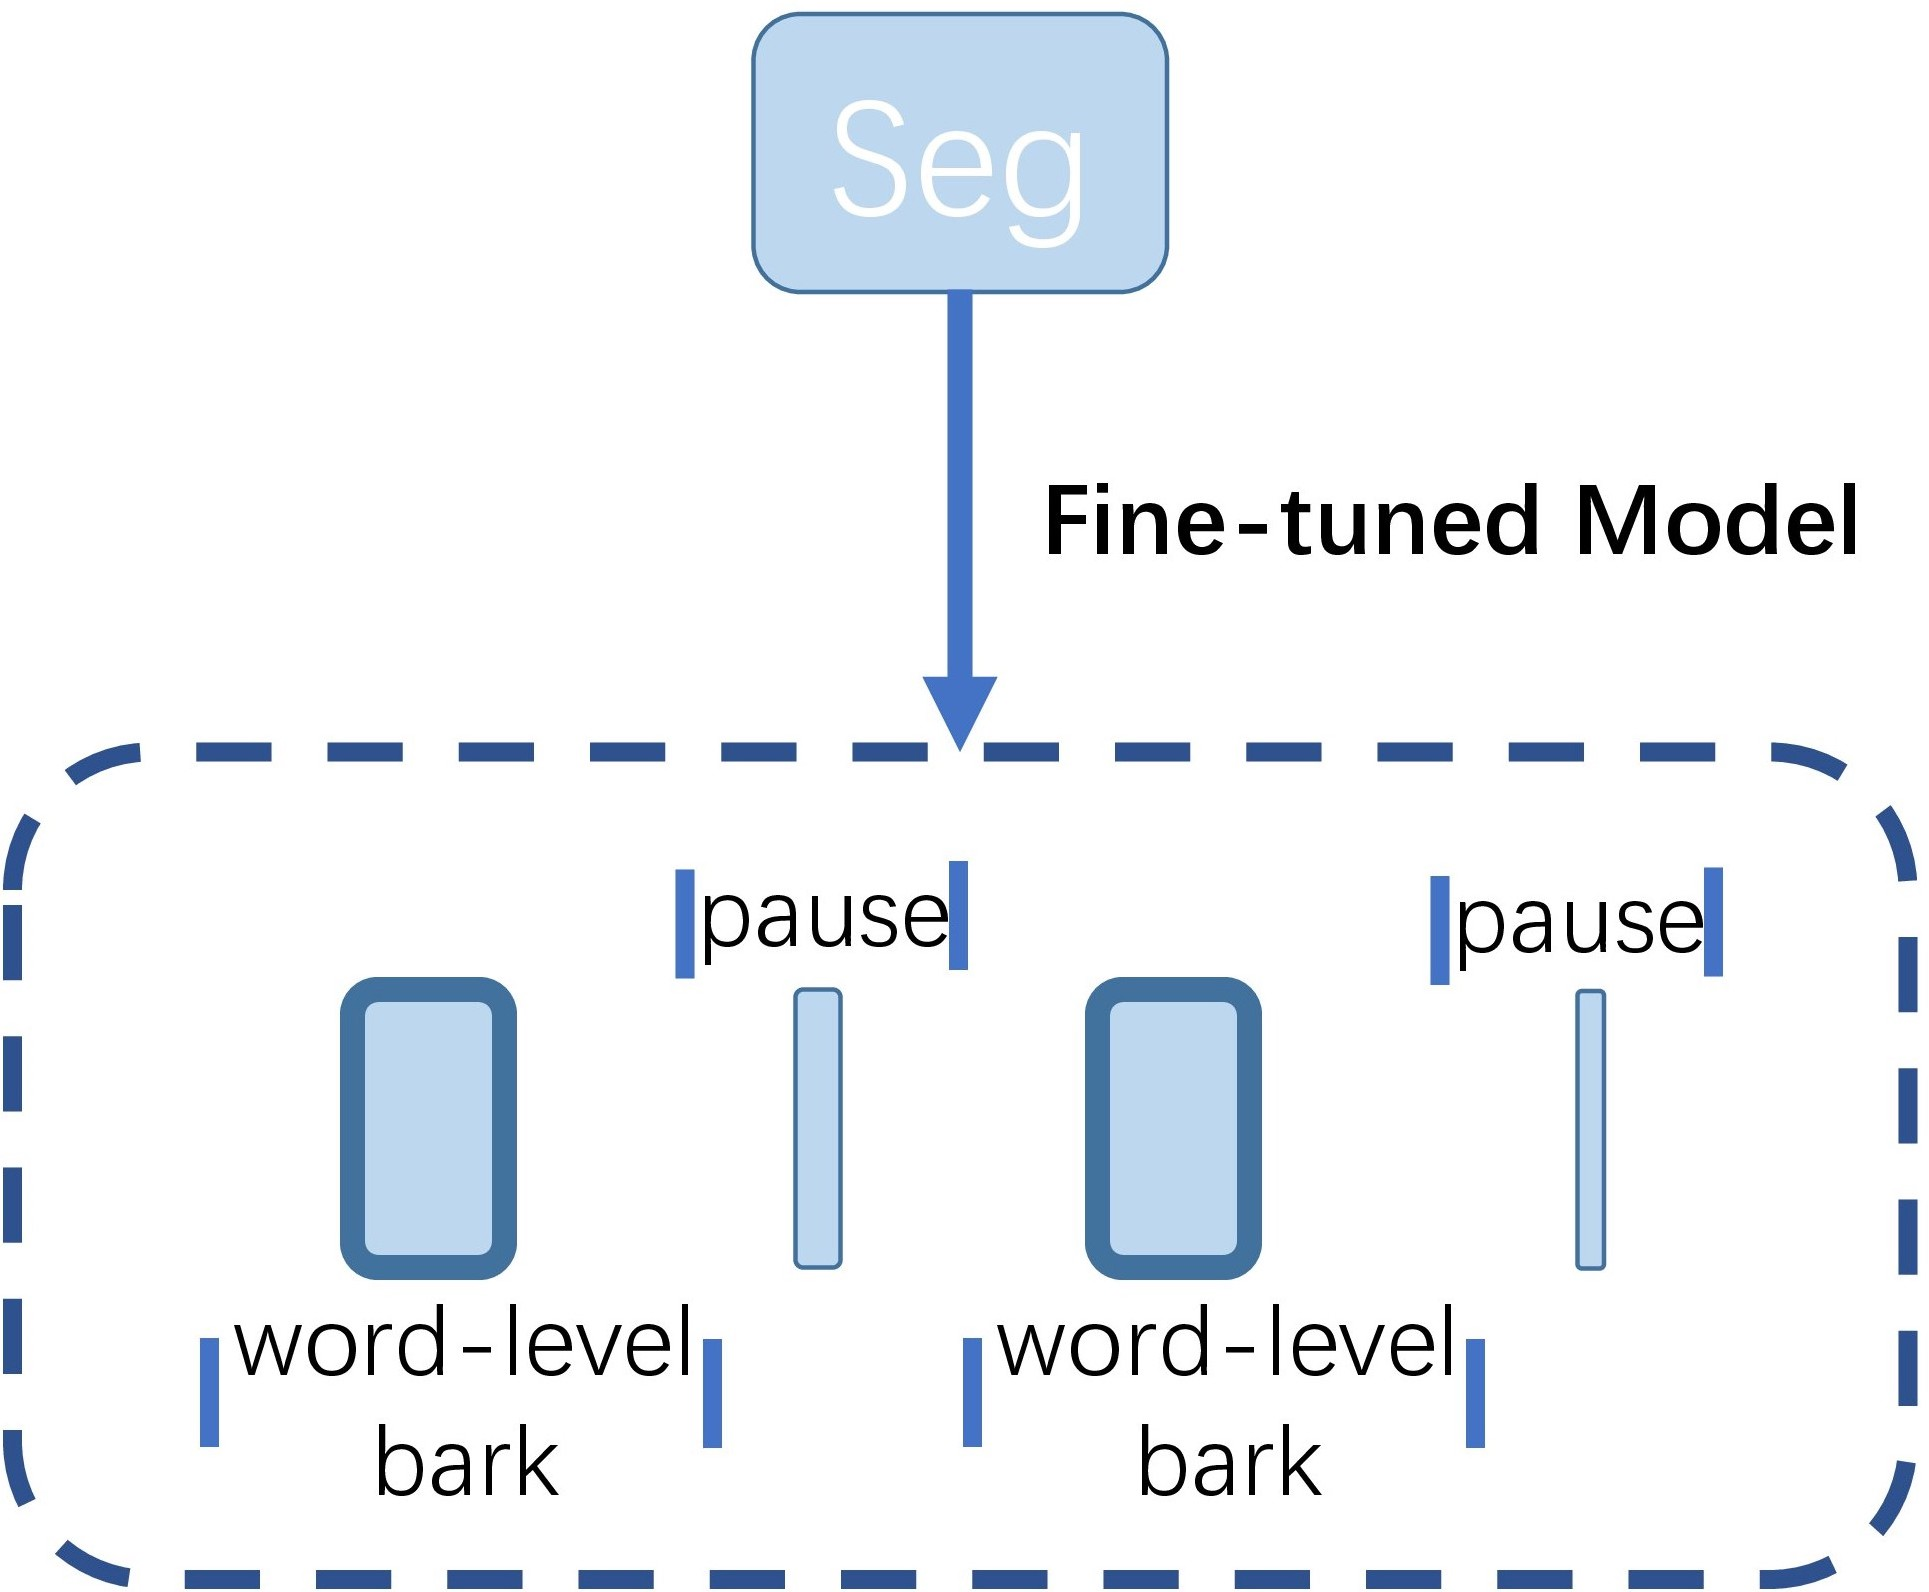
\includegraphics[width=0.98\columnwidth]{images/image3.jpg}
	\caption{word-level barks.}
        \label{fig:word}
\end{subfigure}
\begin{subfigure}[t]{0.7\columnwidth}
        \centering
        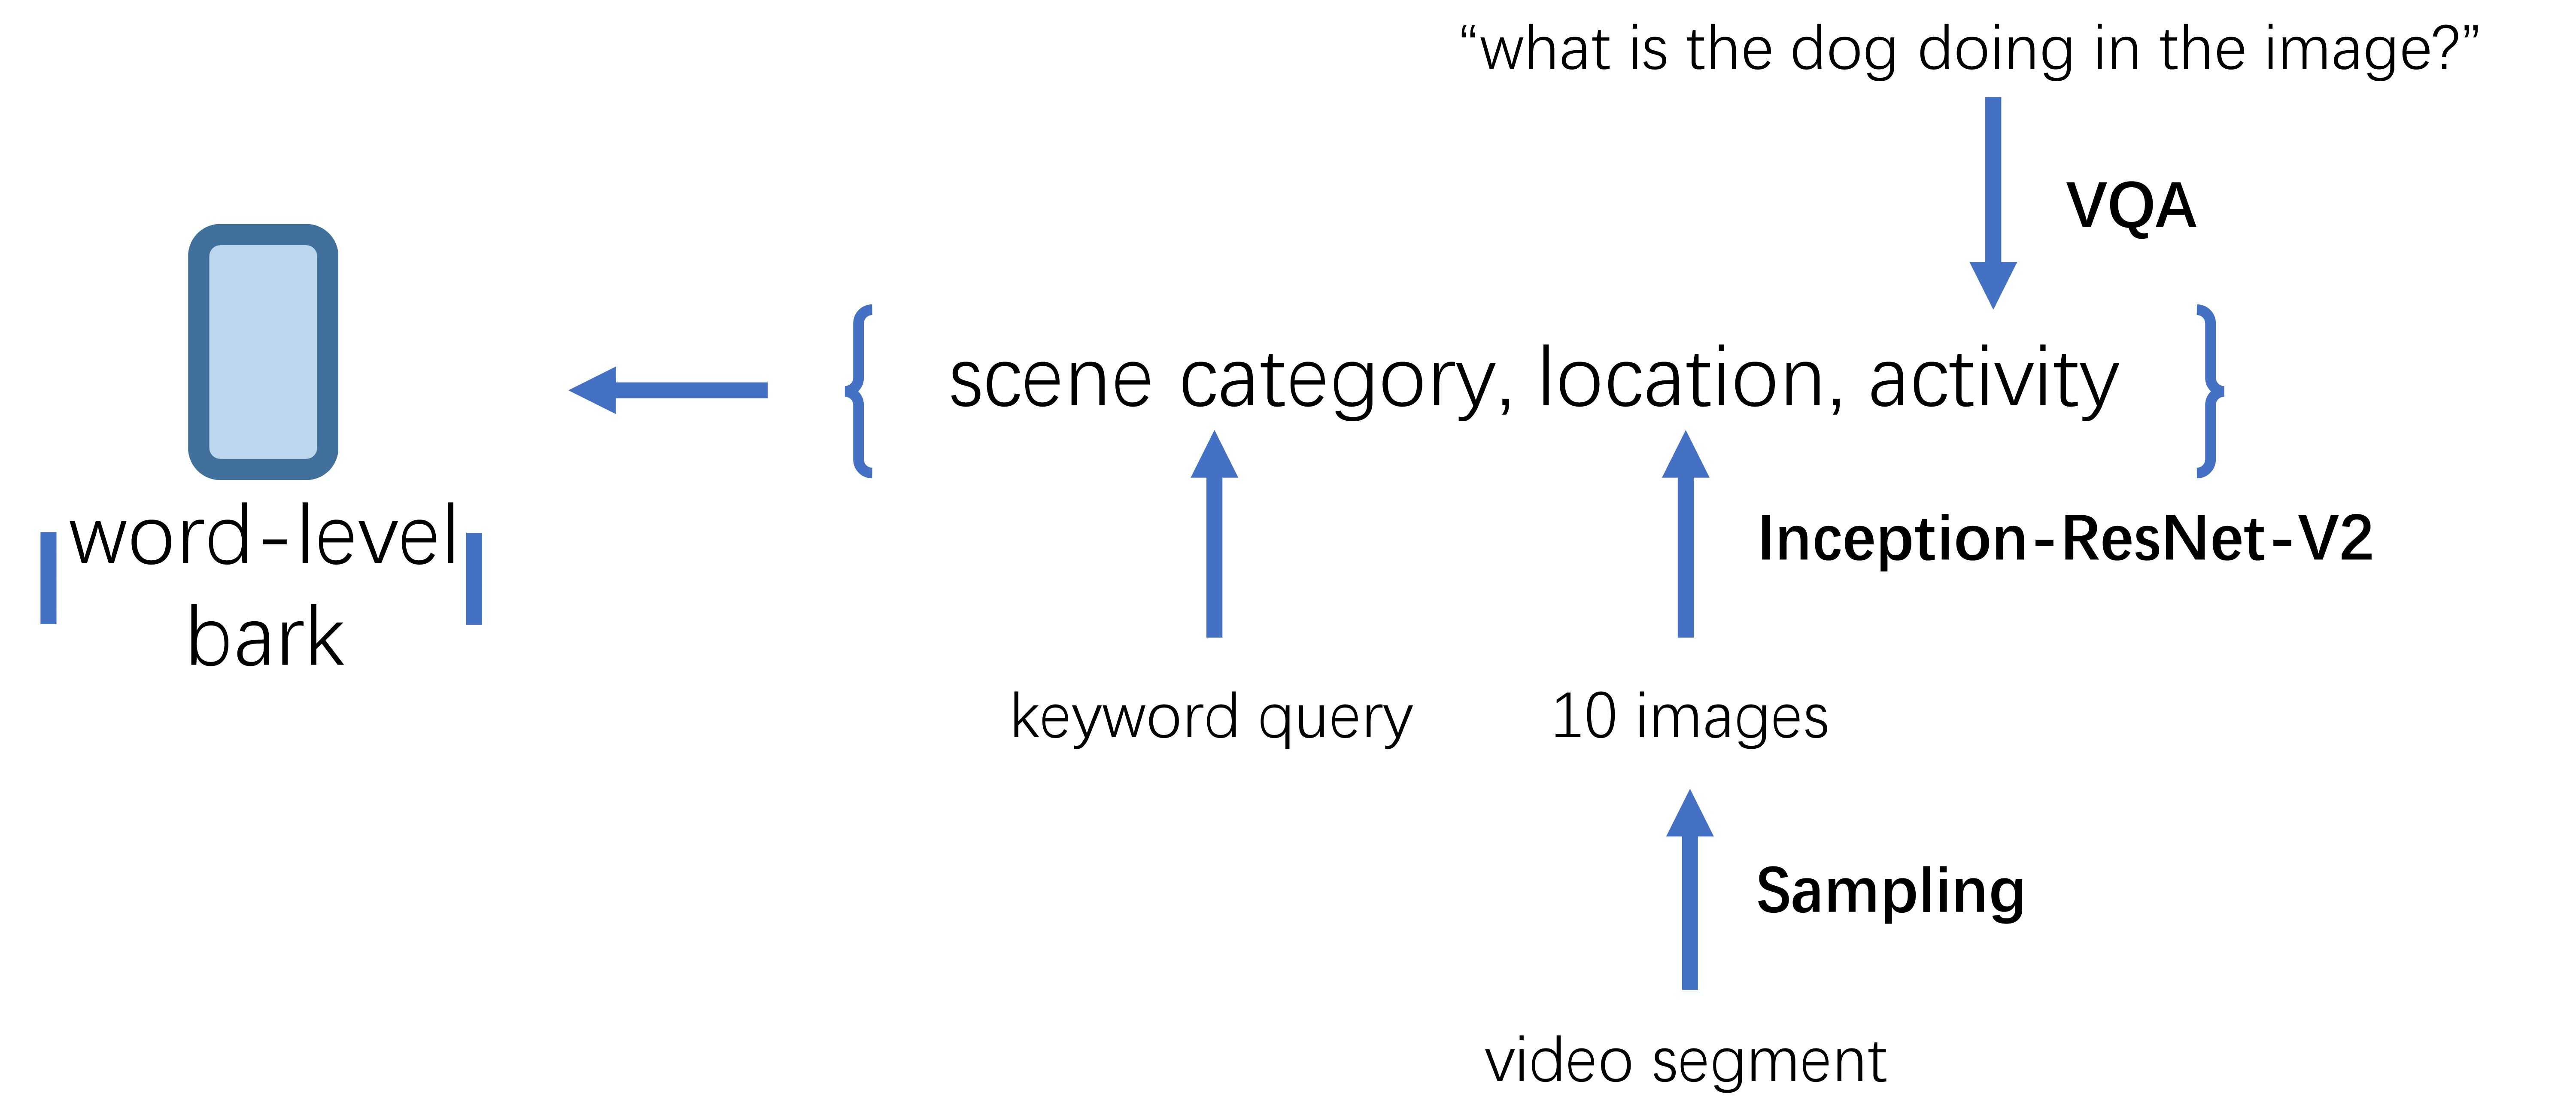
\includegraphics[width=0.98\columnwidth]{images/image4.jpg}
	\caption{context tagging.}
        \label{fig:context}
\end{subfigure}
\caption{The procedure of dataset construction.}
\label{fig:methodpic}
\end{figure}

 
\subsection{Sourcing Dog Vocalization Sounds Online}
\label{sec:source}
Since YouTube contains a large amount of user-uploaded videos about their pet dogs, our first step is to source relevant clips from two language environments via searching for the keyword
``Shiba Inu'' and a scene category term on YouTube. In this study, we use a total of eight scene
categories, which are defined in \tabref{tab:context}. These eight categories were proposed
in previous work about dog activity classification~\cite{larranaga2015comparing}. 
For example, to download videos about Shiba Inu eating, we search for
the query ``Shiba Inu Eat -Coin'' for English and the correponding Japanese of this query for vocals under Japanese host language environment. Here ``-Coin'' is used as there are a large number of Shiba Inu Coin videos, we add this term to filter out those irrelevant videos. All eight scenes are searched under the same keyword patterns.

Because YouTube videos are not typically tagged with original language or locale, we infer the language environment of a video by the languages ofits caption or title. For example, if the title contains Japanese characters, we consider it as a video recorded in an Japanese-speaking environment, whereas a video with purely English title is considered to be recorded in an English-speaking environment. 

After all the videos are downloaded and tagged, 16,161 videos in total are collected. Among them we randomly sample 1,000 clips to verify the host language tagging accuracy by watching the video clips. The accuracy is 93.2\%, which indicates that the majority of the Shiba Inu videos are tagged with the correct host language environments, and fit our research purpose.




\subsection{Dog Vocalizations Extraction}
\label{sec:barkextraction}
The original audios downloaded from YouTube contain long uninformative segments where dogs are silent or background noises muffling the vocalizations. To ensure the quality of 
our dataset, we have adopted a systematic and rigorous pipeline of three steps 
to extract pure and singular vocal segments from the audios.


\paragraph{Step 1: sentence-level segmentations extraction}
As a preliminary step, we extract long segments in which contains a continuous series of
dog vocalizations. Such long segments, which we call a dog ``sentence'', can be detected because
they are preceded or followed by significant periods of silence. 
We apply PANNs~\cite{kong2020panns}, a pre-trained large sound 
event detection model including as many as 527 sound classes for recognizing the 
sound events. The continous segments detected by PANNs with the event class ``barking'' are considered as the sentence-level bark segmentations.
\paragraph{Step 2: noise elimination}
From our practical experience, we have found that sometimes vocalizations will be unclear 
due to the background music and human talking. Thus in the second step, 
among those sentence-level segmentations, those with co-existing event ``speech'' and 
``music'' detected by PANNs are removed from the dataset.

\paragraph{Step 3: word-level vocalizations extraction}
Another challenge is that the coarse-grained sound clips may have 
some short pauses in the middle. To remove 
these pauses, we finetune a sound event detection model to 
determine the start and end time of singular vocalizations, which we call ``words'' 
in this paper.

PANNs is used as the pretrained model, which is trained on AudioSet~\cite{gemmeke2017audio} for all the sound classes first. 
We then manually made framewise labels for the event ``barking'' on 246 audio clips with a total length of 715 seconds and fine-tuned this pretrained model.
This fine-tuned model can precisely detect dog vocals in the audio with the start time and end time. Based on the precise start time and end time, we use the fine-tuned model to remove the pause segments between barkings.  

At the end of these three steps, only a singular dog vocalization is left in each clip. 
In total, 7,500 clips from 1,551 raw videos remained. While we acknowledge the fact that the data noise induced by recording devices and audio ambience is difficult to eliminate via web data, such factors/biases should be well mitigated with the large and diverse data source coming from either side of the Pacific that we curated on YouTube.

\subsection{Context Metadata Tagging}
\label{sec:tag}

We list the range of possible values for {\em scene}, {\em location}
and {\em activity}, three components of the context in \tabref{tab:context}. The set of values for locations values is a subset of the location set from Inception-ResNet-V2 model. 
%\KZ{The set of values for locations were previous presented by ??? cite?.}
%the previous study suggests eight scenes that can influence dog barking, listed in the ``Scene'' row of
% \tabref{tab:context}. To ensure that we provide enough contextual information, 
%we add other information as location and activity, which are illustrated respectively in ``Location''(second row, \tabref{tab:context}) and ``Activity'' (third row, \tabref{tab:context}).


\begin{table}[th]
\small
\begin{tabular}{p{0.12\columnwidth}|p{0.8\columnwidth}}
\toprule
\textbf{Context} & \textbf{Possible values} \\ \midrule
Scene & Alone, Bath, Eat, Fight, Play, Run, Stranger, Walk \\ \midrule

Location & 76 possible locations, such as lawn, street, office, recreation\_room and so on \\ \midrule
%Location & bedchamber, residential\_neighborhood, lawn, elevator/staircase, airplane\_cabin, arena/performance, forest, hospital, igloo/ice\_engraving, farm/farm\_field, recreation\_room, lake/river, pasture, dining\_room, street, balcony, ocean/beach, office, countryside, nursery, art\_room, gymnasium, museum, kitchen, firefighting, library/bookstore, racecourse, coffee\_shop, repair\_shop,  beauty\_salon, desert/sand, landfill, mountain, bowling\_alley, rodeo, greenhouse, aqueduct, ski\_slope, conference\_room, aquarium, boxing\_ring, music\_studio, athletic\_field, auto\_showroom, garden, laboratory, plaza, swimming\_pool, general\_store, raft, orchard/vegetable, campsite, amusement\_park, bridge, airport\_terminal, assembly\_line, station/platform, construction\_site, landing\_field, clothing\_store, banquet\_hall, gas\_station, temple/east\_asia, classroom, discotheque, soccer\_field, bar, skating\_rink, palace, tower, baseball\_field, ticket\_booth, television\_studio, golf\_course, pavilion, church \\ \midrule

%Location & bedchamber, residential\_neighborhood, elevator/staircase, lawn, airplane\_cabin, arena/performance, forest, hospital, igloo/ice\_engraving, farm/farm\_field, recreation\_room, lake/river, pasture, dining\_room, street, balcony, ocean/beach, office, countryside, nursery, art\_room, gymnasium, museum, kitchen, firefighting, library/bookstore, racecourse, coffee\_shop, repair\_shop,  beauty\_salon, desert/sand, landfill, mountain, bowling\_alley, rodeo, greenhouse, aqueduct, ski\_slope, conference\_room, aquarium, boxing\_ring, music\_studio, athletic\_field, auto\_showroom, garden, laboratory, plaza, swimming\_pool, general\_store, raft, orchard/vegetable, campsite, amusement\_park, airport\_terminal, assembly\_line, station/platform, construction\_site, landing\_field, clothing\_store, bridge, banquet\_hall, gas\_station, temple/east\_asia, classroom, discotheque, soccer\_field, bar, skating\_rink, palace, tower, baseball\_field, ticket\_booth, television\_studio, golf\_course, pavilion, church \\ \hline
Activity & a 768-dimentional real valued vector \\ 
\bottomrule
\end{tabular}
\caption{Description of the context metadata. %\KZ{Fill in the blanks in this table.}
}
\label{tab:context}
\end{table}


For locations and activites, we sample 10 images (equi-spaced) from the video segment that 
coincides with the duration of the audio bark sample, and classify the images into one of the location labels listed in \tabref{tab:context}. The locations are inferred from Inception-ResNet-V2 model\cite{szegedy2017inception} trained on AI Challenge 2017 Scene Classification dataset. We apply image caption and visual question answering (VQA) models from OFA~\cite{wang2022unifying} to first generate a caption for an image and then ask the model ``what is the dog doing in the image?''. The caption results are transformed into word embeddings with pre-trained BERT model\cite{devlin2018bert}, and the 10 word embeddings of the 10 images are averaged to obtain the overall activity embedding of that bark sample. Besides, the timestamp of each bark clip in the original video is provided. Some samples from this dataset are shown in \figref{fig:EJShiba}.




\begin{figure}[th]
	\centering
	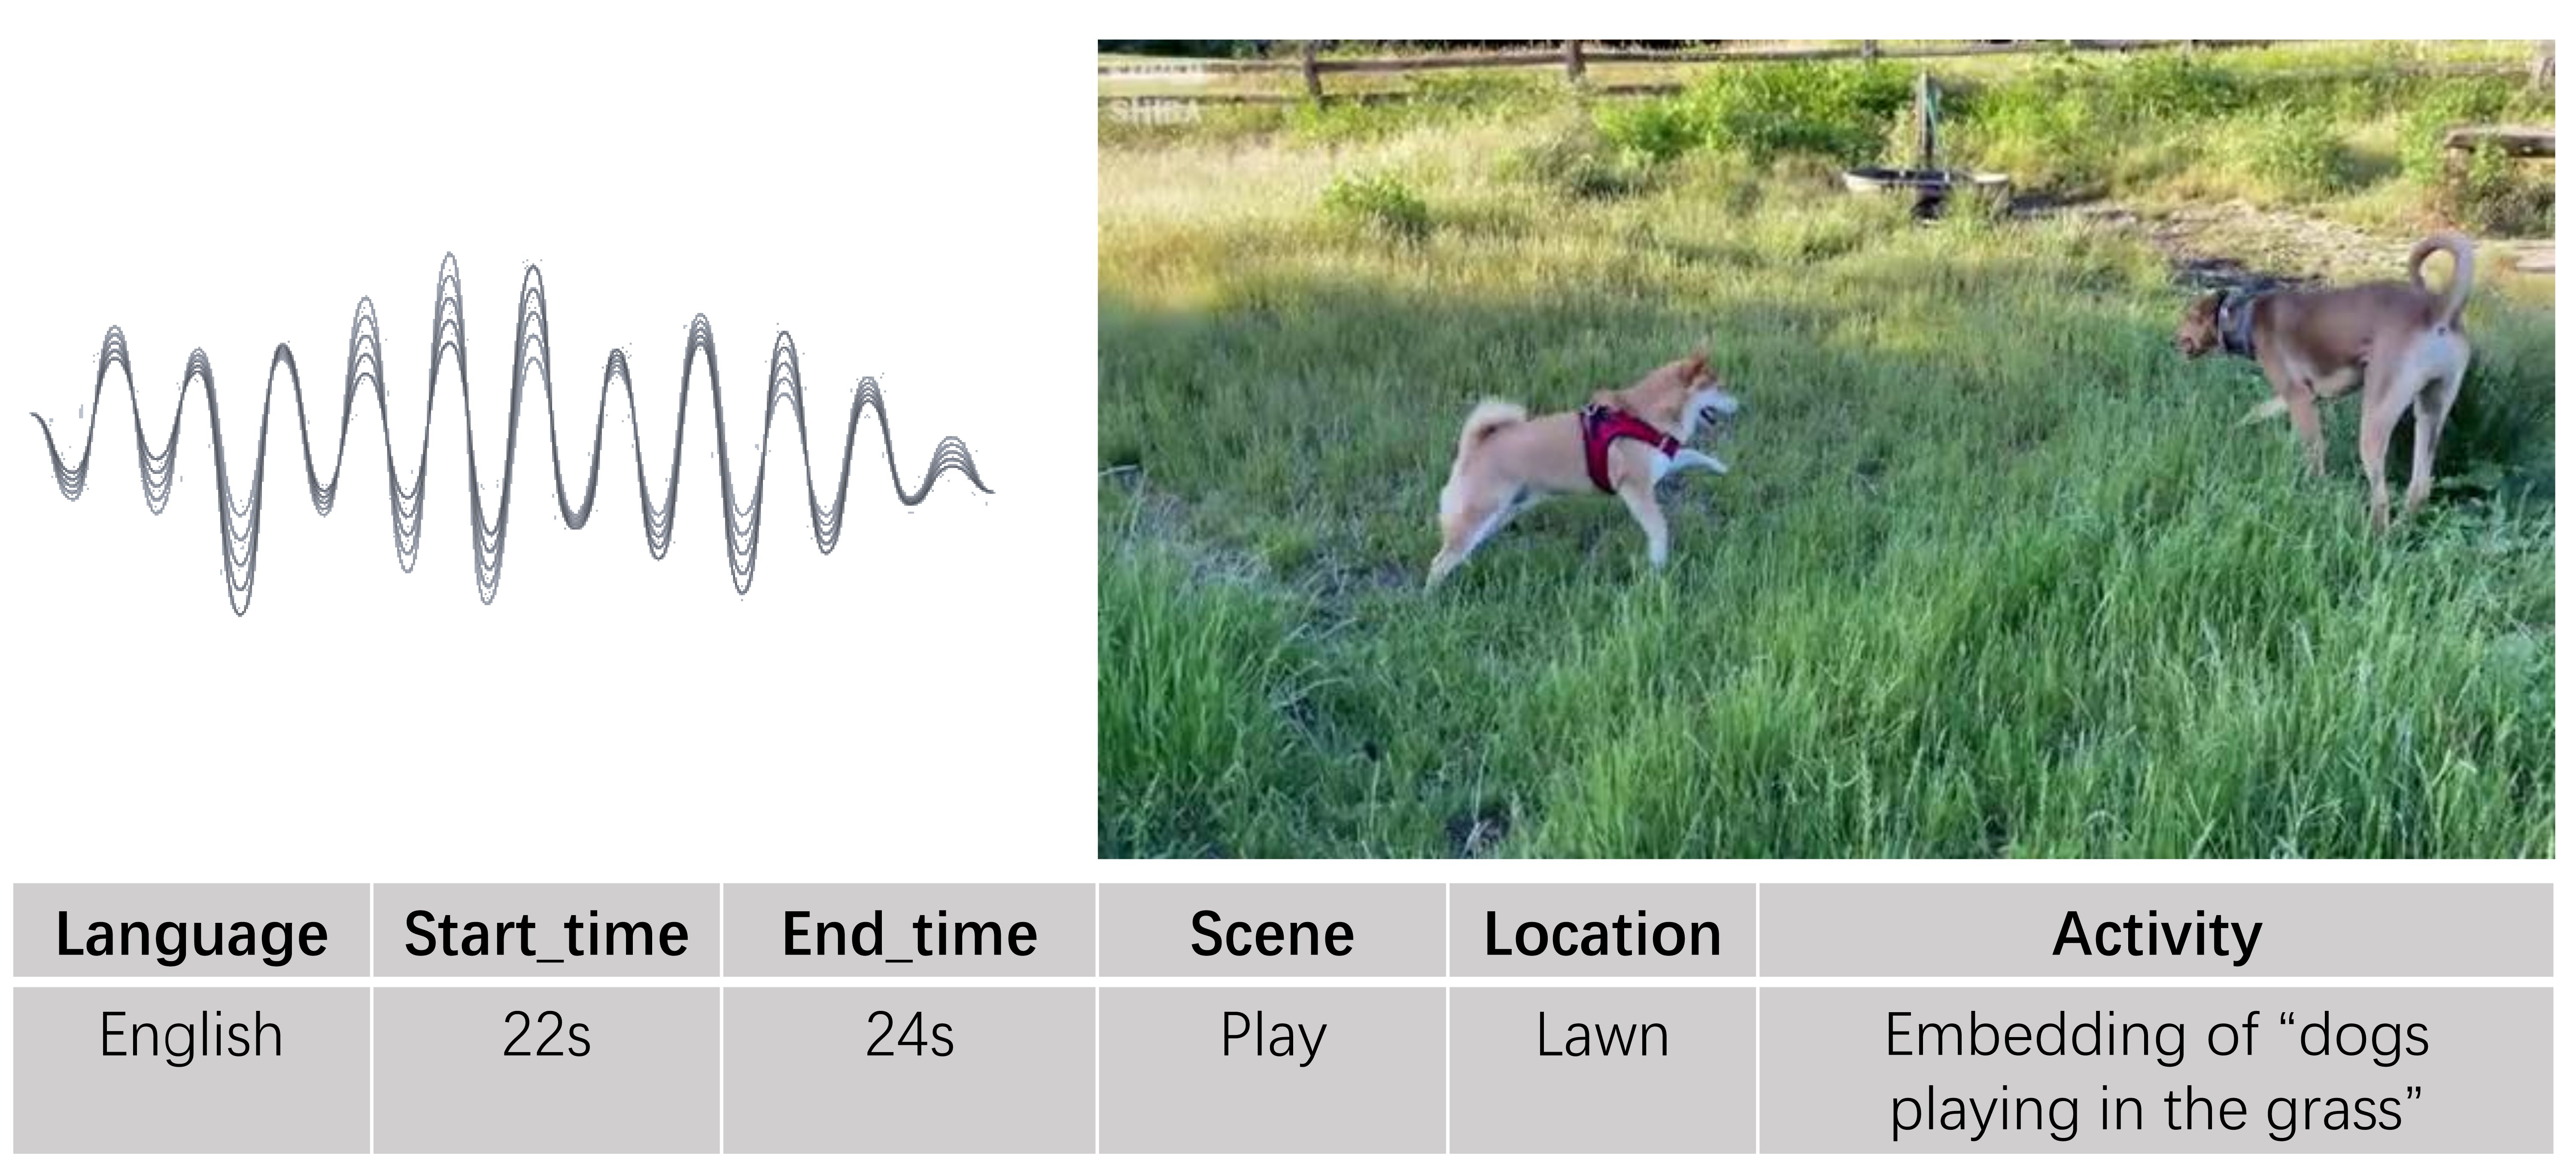
\includegraphics[width=\columnwidth]{images/sample.jpg}
	\caption{One audio sample in EJShibaVoice with its metadata of language environment, 
timestamps, and context.} 
	\label{fig:EJShiba}
%	\Description {One sample in our dataset.}
\end{figure}


\subsection{Host Speech Extraction}
\label{sec:speechextraction}
To address the second research question, which is to find
the correlation between the barks and their host languages, 
we need the audio speech data from dogs' hosts as well. 
The human speech in the original audio track is also extracted by a 
strict pipeline. The first few steps are similar to dog barking extraction: 
we start by getting those continuous segments tagged as ``speech'' by PANNs and 
remove those tagged as ``music'' from them to reduce the noises. As it is normal for several people talking simultaneously, we further apply a speaker diarization 
model Pyannote\cite{Bredin2020, Bredin2021} to separate them from each other and retain speech of a single person 
in more fine-grained segments.

\subsection{The Final Product}
The dataset consists of two parts: the barks and the corresponding host speech. After the whole processing, 7,500 clean bark sounds and 15,197 corresponding host speech clips 
finally remain in our EJShibaVoice dataset~(\tabref{table:datasetlength}).

\begin{table}[th]
	\tiny
	\centering
	\begin{tabular}{c|c|c|c|c}
		\toprule
		{}            & \# of Clips & Avg Len (s) & Var of Len ($s^2$) & English Per(\%)\\
		\midrule
		{Bark} & 7500 & 0.61  &  0.288 & 46.72\\
		{Speech} & 15197 & 1.56 & 2.134 & 44.01\\
		\bottomrule
	\end{tabular}
	\caption{EJShibaVoice Statistics.
%\KZ{maybe instead of showing the num of clips from english env, show a percentage?}
}
	\label{table:datasetlength}
\end{table}

As the data statistics indicate, we include roughly equal number of audio clips 
from English and Japanese environments, leading to a balanced dataset that can well 
support our investigation on the influence of language environment.

The number of clips of each scene differs~(\figref{fig:keyword_rosepie}). 
As we use the same method to process each scene, the possible reason for imparity is that Shiba Inu barks diversely under different conditions. For example, dogs tend to bark more
to show their strength when fighting, therefore the number of clips under ``fight'' is 
the largest.


\begin{figure}[th]
	\centering
	\scalebox{0.2}{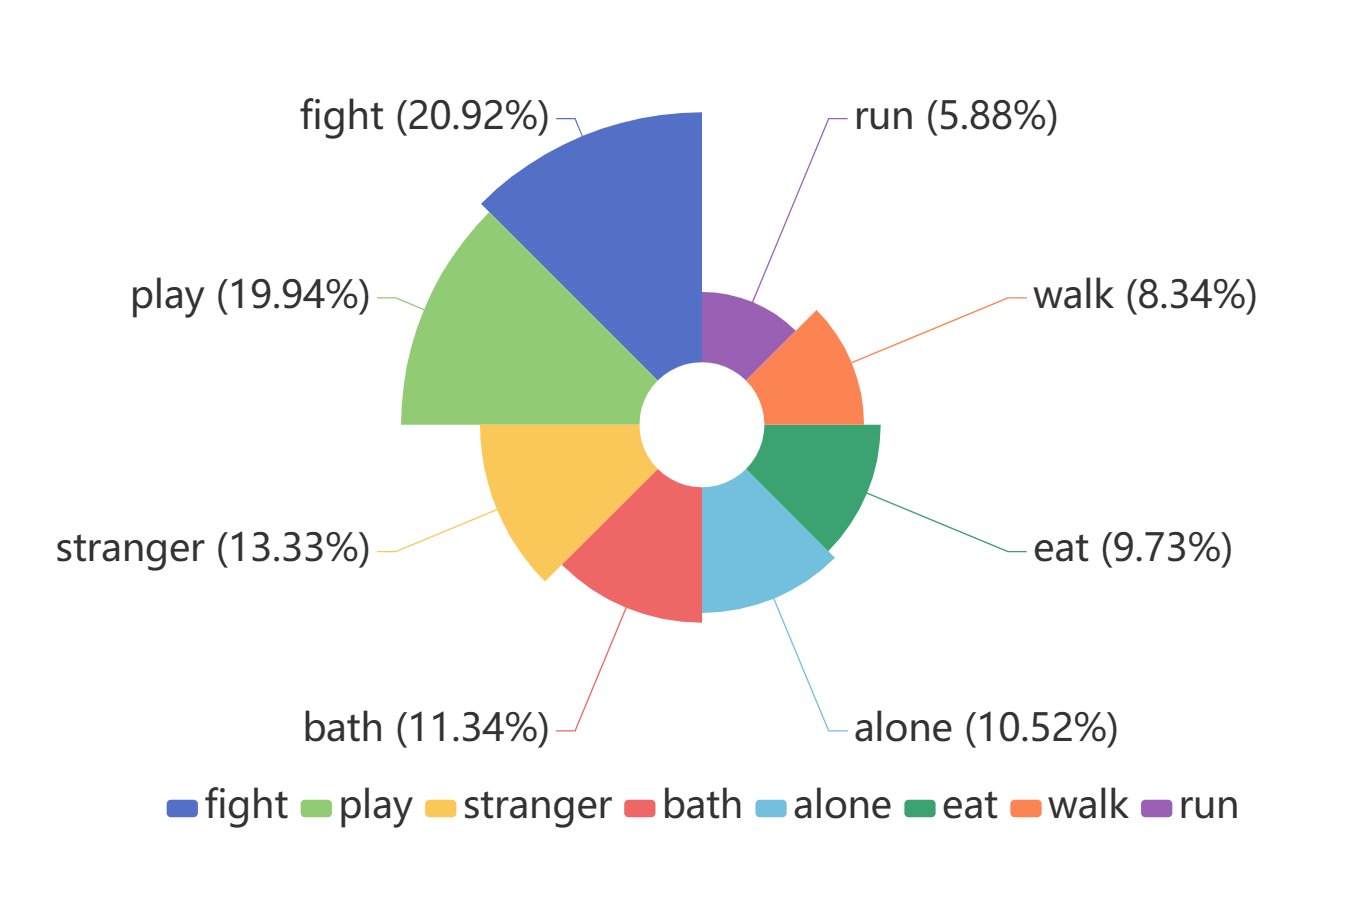
\includegraphics{images/pierose.png}}
	\caption{The percentage of bark clips for different scenes.}
	\label{fig:keyword_rosepie}
%	\Description {The number of bark clips for different scenes.}
\end{figure}
